\documentclass[fleqn,10pt]{wlscirep} 

\usepackage{setspace}
\usepackage{lineno}
\doublespacing


%%%% (20 words or less)
\title{Genotypic variation in foundation trees generates ecological
  network structure}


\author[1,2,*]{Matthew K. Lau}
\author[2]{Louis J. Lamit}
\author[3]{Rikke R. Naesbourg}
\author[4]{Stuart R. Borrett}
\author[1]{Thomas G. Whitham}

\affil[1]{Department of Biological Sciences and Merriam-Powell Center
  for Environmental Research, Northern Arizona University, Flagstaff,
  AZ 86011, USA}
\affil[2]{Harvard Forest, Harvard University, 324 N Main St,
  Petersham, MA 01366, USA}
\affil[3]{University of California Berkeley, Berkeley, CA, USA}
\affil[4]{Department of Biology and Marine Biology, University of
  North Carolina Wilmington, 601 South College Road, Wilmington, NC,
  28403, USA}


\affil[*]{matthewklau@fas.harvard.edu}

%% \affil[+]{these authors contributed equally to this work}

\keywords{Keyword1, Keyword2, Keyword3}

\begin{abstract}
Biological evolution is argued to occur in the context of complex
networks of interacting species in which natural selection defines the
structure of ecological networks \cite{Rezende2007, Guimaraes2011,
  Moya-Larano2011, Thompson2014, Fortin2017}. However, fundamental to
this evolutionary process is the discovery of a genetic basis to
ecological network structure, which remains unknown.  Here, we use
both a long-term experimental common garden \cite{Martinsen2001} with
genotyped individuals and a natural riparian forest of the foundation
tree species \cite{Ellison2005} \textit{Populus angustifolia}, to test
how genetic variation contributes to the interaction network structure
of a model community comprised of epiphytic lichens. We found three
main results:  1) lichen communities showed significant unipartite
(i.e., one mode) network structure that was similar between the common
garden and a natural stand, 2) individual tree genotype significantly
influenced lichen species interactions, which was strongly correlated
with bark roughness, a genetically based trait known to influence
epiphytic lichen \cite{Winfree2011}, and 3) bipartite (two mode)
genotype-species networks, comprised of the foundation species and its
associated lichen community, showed significant modular structure in
both the common garden and natural stand. These results demonstrate
strong support for a genetic basis to ecological network structure and
the potential for selection to act in complex ecosystems. This work
sets the stage for studies that address greater complexity in the
evolution of biological systems and provides a framework for the
discovery of evolutionarily dynamic compartments in ecosystems.

\end{abstract}

\begin{document}

\flushbottom
\maketitle
% * <john.hammersley@gmail.com> 2015-02-09T12:07:31.197Z:
%
%  Click the title above to edit the author information and abstract
%
\thispagestyle{empty}

%% \noindent Please note: Abbreviations should be introduced at the
%% first mention in the main text – no abbreviations lists. Suggested
%% structure of main text (not enforced) is provided below.

\linenumbers

\section*{Introduction}

Evolution occurs in the context of complex networks of interacting
species. In ecological communities, community dynamics depend on key
interactions \cite{Fontaine2011} that occur in species interaction
networks, such as:  trophic \cite{Bascompte2006} and mutualistic
\cite{Rafferty2013} interaction networks. Phylogenetic patterns in
ecological networks support the importance of evolutionary processes
in shaping species interactions \cite{Rezende2007,
  Whitham2006a}. Community genetics studies \cite{Lamit2011} have
shown that genetic variation in foundation species \cite{Ellison2005}
(species, such as trees, that largely define the composition of
communities by creating locally stabile conditions and modulating
resources; contributes to variation in interactions with dependent
communities in both terrestrial and aquatic ecosystems
\cite{Bailey2009a}. more specifically, genetic variation affects
diverse chemical, phenological, morphological and other traits
producing a multivariate phenotype \cite{holeski2012} that makes each
individual unique so that different communities assemble on different
genotypes resulting in different species interaction
\cite{whitham2012, burkle2013}.

although, some empirical studies have shown that genetic variation in
a single species can impact a tri-trophic interaction
\cite{smith2011}; currently no studies have yet investigated the
impact of intraspecific genotypic variation on network structure,
which is integral to the process of evolution by natural selection.

\textbd{add newer lit studies here.}
\begin{itemize}
\item McKnight's paper
\item Arts 2017 paper
\item Daves 2016 paper
\item Jamie's 2016 paper
\item Nat Eco Evo 2017
\item Liza and Amy 2017
\item Ghering 2017
\item Poisot
\item Josh ???
\end{itemize}



Here, we investigate how genetic variation in a foundation tree
species determines the structure of a network of interactions among
species. Using a long-term (20 years+), common garden experiment with
replicated individuals of known genetic identity and a naturally
established stand of \textit{P. angustifolia}. We focused on a model
community of 9 epiphytic lichens species, as previous research has
demonstrated significant compositional responses of epiphytes to
genotypic variation \cite{Winfree2011, Zytynska2011}. In addition, the
ecology of lichen, with local interactions and slow population
turnover rates, allowed us to assess interactions among lichen species
rapidly on individual trees.



\section*{Results}

%%% Up to three levels of \textbf{subheading} are permitted. Subheadings should not be numbered.

In both the experimental garden and the natural stand, we discovered
that genotypic variation in a \textit{P. angustifolia} predictably
influenced the structure of the lichen species interaction network and
contributed to the formation of evolutionary modules comprised of tree
genotypes and the lichen community.  We observed significant
unipartite (one-mode) network structure \cite{Araujo2011} in the
lichen species interaction networks that was similar between the
experimental garden and the natural stand (Fig. 1a and 1b; Garden: z =
-6.31, p = 0.0002; Natural: z = -3.15, p = 0.002). The two networks
displayed high multivariate structural similarity (Mantel R = 0.51, p
= 0.029). Node level eigen-centrality \cite{DeAngelis1989}, a measure
of species importance that integrates indirect connections, showed
strong correlation between the two stands (Fig. 1c; r = 0.7, t =
2.6135, df = 7, p = 0.035). Centrality was also highly correlated with
total abundance in both networks (Fig. 1d; Garden: r = 0.77, t =
3.2427, df = 7, p = 0.014; Natural:  r = 0.86, t = 4.43, df = 7, p =
0.003). In combination, the similarity of both the whole and node
level network structure between the common garden and the wild
indicates that the common garden environment captures much of the
natural variation that exists in nature and accurately reflects
natural processes.

In the common garden, where the effect of environmental variation was
controlled, genotype was an important factor contributing to network
structure. Genotype was a significant predictor of interactions on
individual trees (Fig. 2a; F = 3.4213, num df = 12.000, denom df =
14.668, p-value = 0.01426). Similar to the effect of a genetically
controlled trait (bark roughness) on a dominant lichen
\cite{Ellison2005}, we found that individual tree genotypes with
similar levels of bark roughness had similar levels of lichen
interactions (Fig. 2a; Mantel R = 0.08, p = 0.013), which was similar
to the correlation observed between bark roughness and lichen
interactions in the natural stands (Fig 2b: r = -0.53, p = 0.050).

We also examined how \textit{P. angustifolia} genotypic
differentiation contributes to the formation of groups of tree
genotypes and lichen species and found significant modular
structure. Using a bipartite (two-mode) network approach in which
genotype-species networks were modeled using the species maximum
relativized values of each lichen species across all
\textit{P. angustifolia} genotypes, we found significant modularity in
the common garden stand (Fig. 3a; z = 9.64, p < 0.001). When using the
same analyses on individual trees in the natural stand, we also found
significant modularity (Fig. 3b; z = 7.42, p < 0.001). Furthermore,
nestedness of both of these networks was significantly lower than
expected under a null model (Garden: z = -2.30, p < 0.001; Natural
Stand: z = -2.84, p < 0.001), most likely as a result of module
formation.  



\section*{Discussion}

%%% The Discussion should be succinct and must not contain subheadings.

These findings support the hypothesis that genotypic variation in a
foundation species can contribute to the structure of a network of
interacting species. Several lines of evidence support this
conclusion. First, the wild stand showed significant interaction
network structure (Fig. 1a and b); and both tree genotype and the
genetically based tree trait, bark roughness, was a strong predictor
of co-occurrence patterns (Fig. 2a). Second, the common garden network
(Fig. 1b) structure showed a high degree of similarity to the wild
stand network structure (Fig. 1c and d). Third, tree genotype was a
significant predictor of SES values (Fig. 2a), displaying significant
correlation with a genetically linked trait, bark roughness, both in
the common garden (Fig. 2a) and in a naturally established stand of
trees (Fig. 2b). Last, both of the bipartite genotype-species networks
in the common garden and natural stand displayed significant
modularity, suggesting that genotypic variation is leading to the
formation of evolutionarily dynamic compartments within the
community. Thus, just as numerous studies have shown that plant
genotype can affect species richness, abundance, diversity, and
composition and previous work has demonstrated that evolutionary
processes shape ecological networks \cite{Guimaraes2011,
  Moya-Larano2011}, our study includes genetics in an empirical
investigation that combines both experimental common garden findings
along with studies in the wild that are in close agreement.

Our results point to the importance of understanding the community
level effects of genetic variation and corroborate previous findings
of the importance of plant genetics in shaping ecosystems
\cite{Whitham2006a}.  This study highlights the potential for indirect
effects of genetic variation to propagate through networks of
interacting species and trophic levels. Altering the structure of
interaction networks presents a means for genetic effects to be
magnified within the system of interacting species. At the scale of
ecosystems, trophic networks or food webs direct and control the rates
of energy and nutrient flux \cite{Borgatti2006}. One important example
\cite{Smith2011}, showed that the interactions among species across
three trophic levels depended on cottonwood (\textit{Populus} spp.)
genotype. Although our study was conducted with a community of
lichens, these results should be generalized to other groups of
diverse organisms around the world that also exhibit significant
genetic signals at the community level \cite{Rowntree2011,
  Whitham2012}, although spatial scale of interactions should be
considered \cite{Zook2010}. As heritable variation is the raw material
for natural selection to act upon, a genetic basis for interaction
network structure indicates evolutionary dynamics should be considered
at the community level and that conserving genetic variation is
important to consider in efforts to restore or preserve complex
species interactions and the associated ecosystem functions
\cite{Evans2013} that they provide.



\section*{Methods}

%% Topical subheadings are allowed. Authors must ensure that their Methods section includes adequate experimental and characterization data necessary for others in the field to reproduce their work.

\subsection*{Field observations in common garden and natural riparian
  forest stands}

The study was conducted along the Weber River, UT (USA), which is a
cottonwood (\textit{Populus} spp.) dominated riparian
ecosystem. Although two native species, \textit{Populus angustifolia}
(James) and \textit{Populus fremontii} (S. Watson), occur here and are
known to hybridize, only pure or highly advanced backcrosses of
\textit{P. angustifolia} were sampled in order to avoid the effect of
the hybridization between these two species.

A common garden setting was used to isolate the effect of tree
genotype from the effect of the localized microenvironment associated
with each individual and spatial autocorrelation. Asexually propagated
clones of genotyped \textit{P. angustifolia} individuals4 were
obtained from wild collections and planted randomly in a single field
(0.025 km$^2$) at the Ogden Nature Center, Ogden, UT in 1992. A total
of thirteen genotypes replicated between 3 and 8 times each, were
chosen for sampling. Genotype names were previously published
\cite{Ellison2005}. Observations were made in the common garden in
October 2010 and May 2011.

The natural stand of \textit{P. angustifolia} near the city of Uintah,
UT (GPS:  N41.13903, W110.94400) was used for the wild stand
survey. We conducted sampling of the stand in May 2012. A total of 14
trees were chosen randomly over a 0.10 km$^2$ area with a minimal
distance of 5.56 m between trees across a range of tree core based
ages from 15 to 60 years.

\subsection*{Bark and Lichen Community Observations}

The bark lichen community in this system is comprised of fourteen
species; however, only 9 species were observed within our study
quadrats. The lichen community included (abbreviations are given for
species present in study): Xg = \textit{Xanthomendoza galericulata},
Xm = \textit{X. montana}, Ch = \textit{Caloplaca holocarpa}, Cs =
\textit{Candelariella subdeflexa}, Rg = \textit{Rinodina glauca}, Lh =
\textit{Lecanora hagenii}, Ls = \textit{Lecanora} (unknown species),
Pm = \textit{Phyciella melanchra}, Pa = \textit{Physcia adscendens},
Pu = \textit{Physcia undulata}, \textit{Phaeophyscia orbicularis},
\textit{Phaeophyscia ciliata}, \textit{Melanelia subolivacea},
\textit{Meanelia elegantula}, including both crustose and foliose
lichen species that exhibit low inter-annual variation
\cite{Ellison2005}. We were able to rapidly assess lichen interactions
by quantifying thalli in closed contact as assessed using 1 cm$^2$
cells. Species accumulation curves showed that communities in the wild
and the common garden were thoroughly sampled and with very similar
species richness (Supplementary Materials). 

On each tree, presence or absence of each lichen species was assessed
in 50 total 1 cm$^2$ cells arrayed in a checkerboard pattern. Two
adjacent 10 cm$^2$ quadrats centered at 50 cm and 85 cm from ground
level were sampled. The checkerboard sampling pattern was chosen to
isolate each cell based on an average thallus size of 1
cm$^2$. Samples were restricted to the northern aspect of the trunk to
maximize the abundance of lichen and control for the effect of
aspect. The thalli in each cell are expected to be spatially
independent of the other cells in the quadrat, but exposed to similar
micro-environmental conditions. Bark roughness was measured on each
tree following \cite{Winfree2011}.

\subsection*{Network modeling and analyses}

We used the observations of lichen in the 1cm$^2$ cells on individual
trees of \textit{P. angustifolia} both in the common garden and the
natural stand. Uni-partite networks were generated using an analytical
procedure that removes non-significant interactions between species
\cite{Araujo2011}. We used a null model based approach for all other
analyses of network structure. A conservative null model that
constrained both the row and column marginal totals was used in order
to account for the effects of variation in species’ total
abundances24. From a total of 5000 null matrices, a standardized score
was calculated for each statistic ($z = \frac{x_{obs} -
  \bar{x}_{sim}}{sd_{sim}}$), including the C-score \cite{Stone1990a},
nestedness \cite{Atmar1993} and modularity \cite{Newman2006}. Here, we
follow the convention of the co-occurrence literature and refer to the
standardized C-Score as the Standardized Effect Size (SES)
\cite{Gotelli2001}.

A correlation test with Pearson’s \textit{r} was used to test for the
correlation between the wild and common garden networks. A Welch
Analysis of Variance (ANOVA), which relaxes the assumption of
homogeneity of variance, was used to test for the effects of genotype
on tree scale SES values. A permutation based Mantel Test was used to
test for the effect of bark roughness on SES values in the common
garden. All analyses were conducted using the programming language R
\cite{RCoreTeam2017}.



\bibliography{Lau_InPrep_Nature}

%% \noindent LaTeX formats cites and references automatically using
%% the bibliography records in your .bib file, which you can edit via the
%% project menu. Use the cite command for an inline cite, e.g.
%% \cite{Figueredo:2009dg}.

\section*{Acknowledgments} 

This work was supported by the National Science Foundation grant
(DEB-0425908) and Integrative Graduate Research Traineeship (IGERT)
fellowships for M.L. and L.L. The Ogden Nature Center staff helped to
maintain the common gardens. Lichen sampling was supported by Todd
Wojtowicz, Luke Evans and David Solance Smith.


\section*{Author contributions statement}

M.L. and L.L. conceived the study, M.L. and L.L. conducted the field
work, R.N.  assisted in lichen identifications, M.L. wrote the first
draft of the manuscript, S.B. and T.W. contributed substantively to
the conceptual development, T.W. established the common garden. All
authors contributed to revisions of the manuscript.

\section*{Additional information}

%% To include, in this order: \textbf{Accession codes} (where applicable); \textbf{Competing financial interests} (mandatory statement). 

%% The corresponding author is responsible for submitting a \href{http://www.nature.com/srep/policies/index.html#competing}{competing financial interests statement} on behalf of all authors of the paper. This statement must be included in the submitted article file.


\clearpage
\newpage

\begin{figure}[ht]
\centering
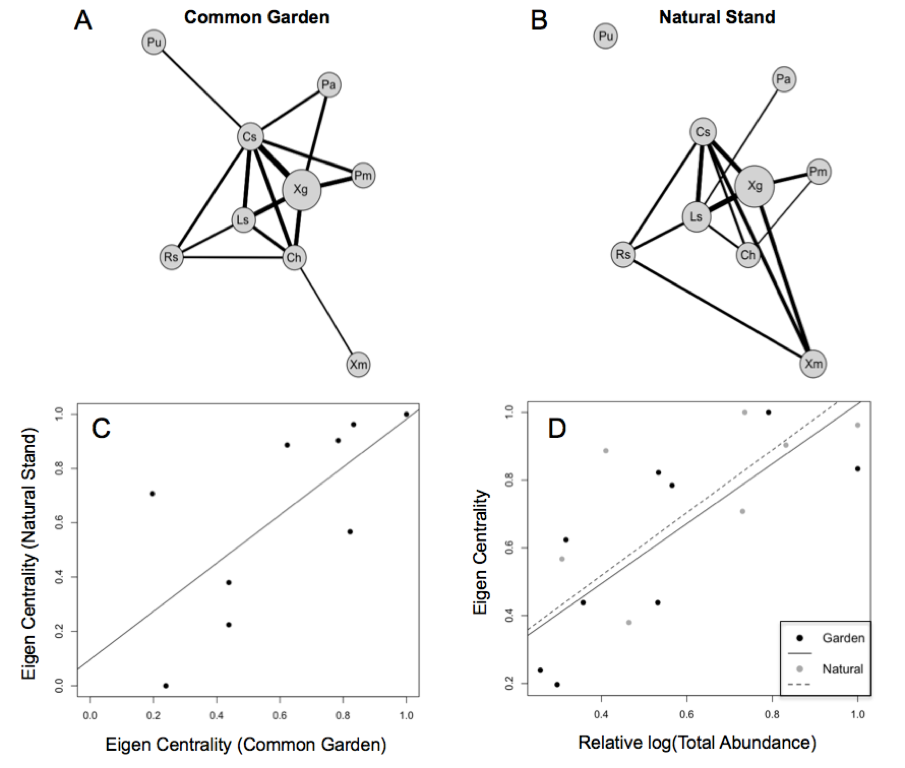
\includegraphics[width=\linewidth]{fig1}
\caption{Significant unipartite network structure was observed for
  epiphytic lichens on trees of known genotype in a common garden (ONC
  = Ogden Nature Center, Utah, USA) (A) and individual trees in a
  natural stand (Uintah, Utah, USA) (B) of the foundation species,
  \textit{Populus angustifolia}. Both networks are shown here with
  lichen species as nodes (see Methods for complete species names)
  scaled by the log of their total abundances and significant
  co-occurrence patterns between species shown as edges scaled by
  their log frequencies. The bivariate plot (C) shows the significant
  correlation in Eigen Centrality between the two networks. (D) The
  total abundance of lichen species was a significant driver of
  network structure for both networks.}
\label{fig:fig1}
\end{figure}

\begin{figure}[ht]
\centering
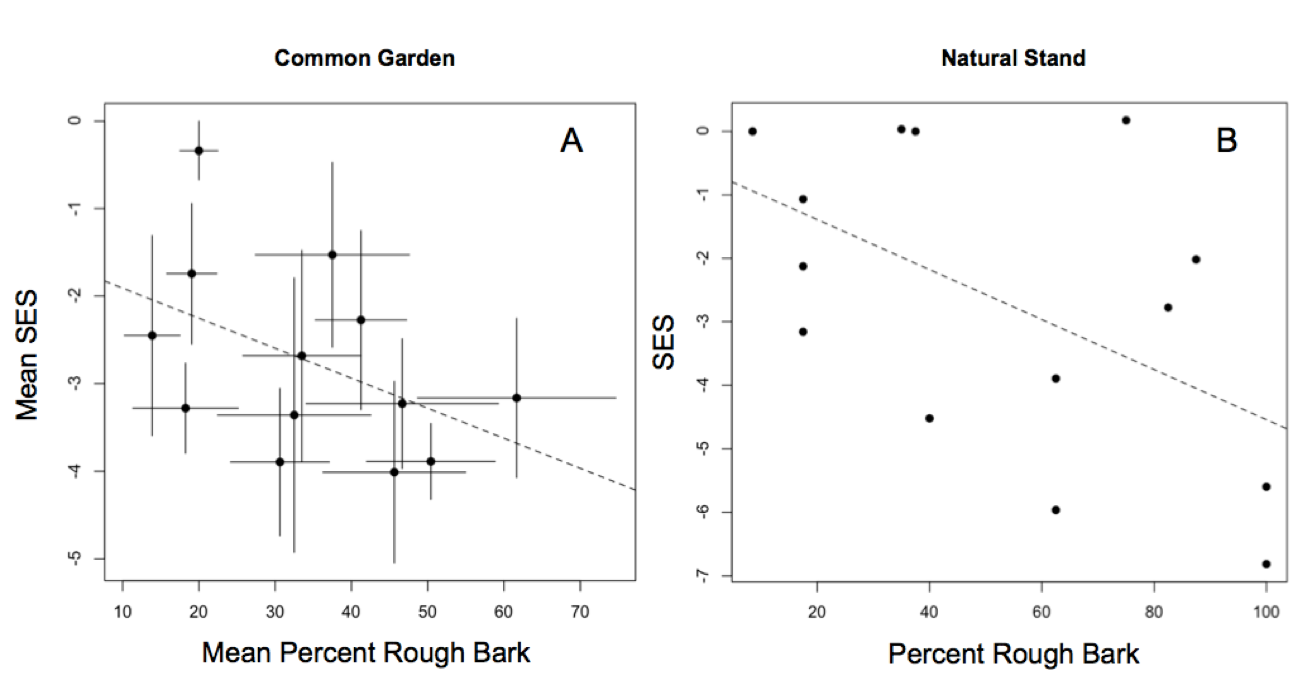
\includegraphics[width=\linewidth]{fig2}
\caption{Tree genotype influenced lichen co-occurrence patterns in the
  common garden and the natural stand through a genetically controlled
  tree trait. The lichen co-occurrence patterns were highly correlated
  with the genetically based phenotypic trait; bark roughness (i.e.,
  the percentage of textured bark), in both the common garden and
  natural stand. The scatterplot (A) shows the mean ($\pm$ 1 SE)
  percent rough bark (broadsense heritability, $H^2$ = 0.36, $\chi^2$
  = 9.214, \textit{p} = 0.002) and SES for each genotype for trees in
  the common garden with SES values becoming more negative (i.e.,
  species interactions increased), indicating stronger co-occurrence
  patterns, as bark roughness increases. The lichen communities on
  individual trees in the Unitah natural stand (B) displayed a similar
  pattern with the SES values becoming increasingly more negative on
  trees with more rough bark.}
\label{fig:fig2}
\end{figure}

\begin{figure}[ht]
\centering
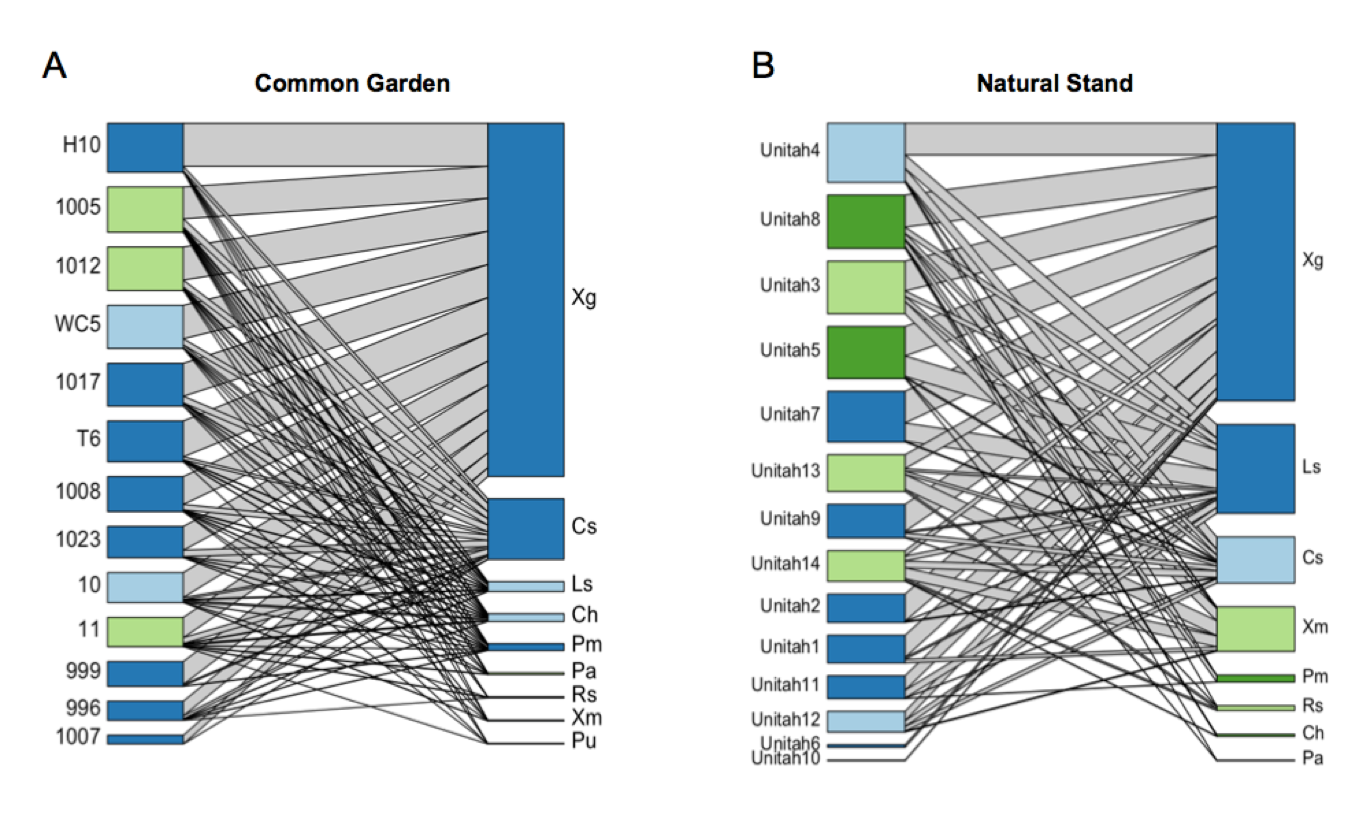
\includegraphics[width=\linewidth]{fig3}
\caption{Bipartite networks displayed significant modularity with
  modules comprised of both genotypes and species. The left most set
  of nodes shows tree genotypes (see Methods for genotype names) for
  the common garden (A) or individuals in the natural stand (B)
  connected to lichen species on the right. Both sets of nodes are
  scaled by their marginal totals (i.e., total observed individuals
  for tree nodes and total abundance for lichen species) and arranged
  by ascending totals from bottom to top. Node color shows the
  significant module membership for both trees and lichen species with
  module color having no direct relationship between the two networks,
  as modules were determined for each network independently.}
\label{fig:fig3}
\end{figure}

%% \begin{table}[ht]
%% \centering
%% \begin{tabular}{|l|l|l|}
%% \hline
%% Condition & n & p \\
%% \hline
%% A & 5 & 0.1 \\
%% \hline
%% B & 10 & 0.01 \\
%% \hline
%% \end{tabular}
%% \caption{\label{tab:example}Legend (350 words max). Example legend text.}
%% \end{table}

%% Figures and tables can be referenced in LaTeX using the ref command, e.g. Figure \ref{fig:stream} and Table \ref{tab:example}.

\end{document}
